\section{RunOff Application}
For the first sprint it was decided the focus should be on creating a very basic application prototype which could showcase the envisioned \ac{GUI} functionality and be able to interface with the server. 

\subsection{User Interface}
At its core the application is intended to be quick and easy to use - the user should open the application, choose a running mode (against friends or against an unknown opponent), pick a route and be ready to go. For the first sprint a rough mockup of the interface for the application was designed, outlined below. The focus was on keeping the navigation level low, i.e. having as much information on each screen as possible to avoid the user having to go through five screens to find the wanted functionality.

When the user opens the application the first screen should show four buttons, encompassing the basic functionality of the application, illustrated in \autoref{fig:mainMock}.

\begin{figure}[!ht]
	\begin{center}
		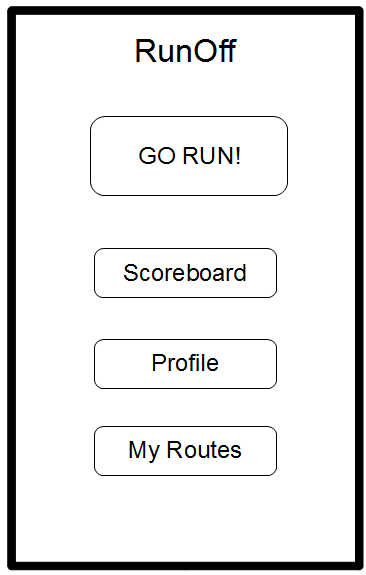
\includegraphics[scale=0.4]{img/mainMockV1.png}
		\caption{Main User Interface Mockup}
		\label{fig:mainMock}
	\end{center}
\end{figure}

The first option is the most vital: start an exercise session. Because this is the main focus of the application this button is larger than the others and the text is written in all caps. The second button takes the user to the Scoreboard where they will be able to see how they compare on a global scale and against friends. This is set as the second option to emphasize the focus on competition to motivate the user to keep running and using the application. The third button shows the user their profile. Here they will be able to see and edit general information such as name, age etc. which will be visible to others, as well as seeing personal records and previously completed runs and their friend list. The last option takes the user to a list of their saved routes showing their distance, difficulty rating, personal best time on the route etc. The user will not be able to edit the routes on the application, for this they need to use the website.

Choosing to start an exercise session will take the user to an options menu shown in \autoref{fig:optionsMock}.

\begin{figure}[!ht]
	\begin{center}
		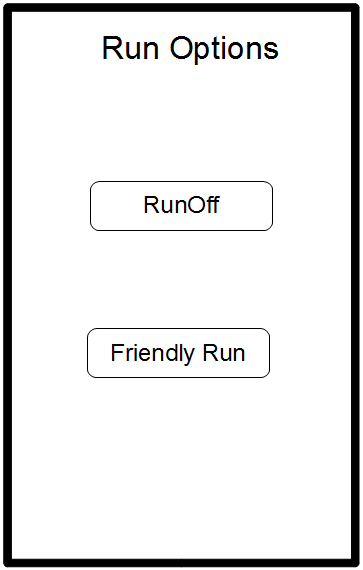
\includegraphics[scale=0.4]{img/optionsMock.png}
		\caption{Options Menu Mockup}
		\label{fig:optionsMock}
	\end{center}
\end{figure}

The user can either choose to start a RunOff, i.e. a ranked game against an unknown opponent, or a Friendly Run against a person on the user's friend list. Choosing either of the two will take the user to very similar screens with the options to pick a route or start looking for a random opponent/choose a friend from the friend list to run against. These screens are illustrated in \autoref{fig:matchMock}.

\begin{figure}[!ht]
	\begin{center}
		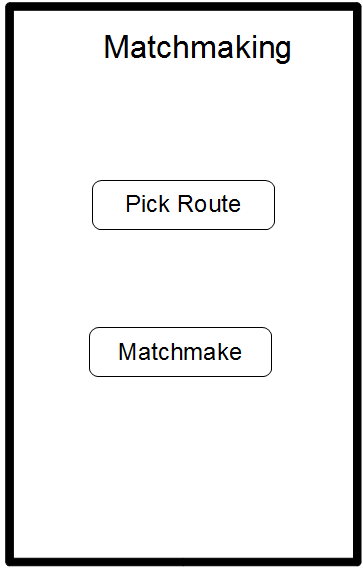
\includegraphics[scale=0.4]{img/matchMock.png}
		\caption{Matchmaking Screen Mockup}
		\label{fig:matchMock}
	\end{center}
\end{figure}

If the user wishes to pick a route, they will push the ``Pick Route'' button which will take them to a list of their saved routes, showing name, distance and difficulty, seen in \autoref{fig:pickRouteMock}.

\begin{figure}[!ht]
	\begin{center}
		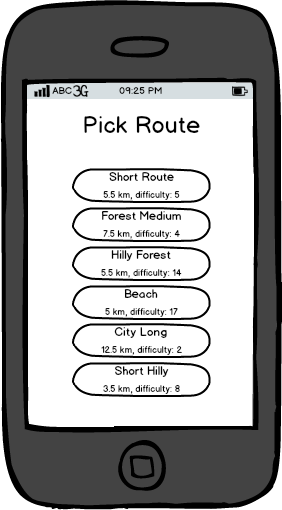
\includegraphics[scale=0.4]{img/pickRouteMock.png}
		\caption{Pick Route Mockup}
		\label{fig:pickRouteMock}
	\end{center}
\end{figure}

\subsection{Implementation}
For the first sprint it was decided that the functionality for the application prototype should be a basic interface and establishing a connection to the server to retrieve the routes created and saved online. The \ac{GUI} was implemented with an activity for each screen and a class to handle the \ac{HTTP} interactions. Implementations of the screens (except the main screen) are trivial as they only handle button clicks and therefore they will not be discussed further in this chapter.

\subsubsection{Main Screen and HTTP Handler}
The main screen, as all the other screens, was implemented as a class extending the \texttt{ActionBarActivity}, with an accompanying \ac{XML} file specifying the layout of the activity. The layout for this activity is shown in \autoref{fig:mainV1}.

\begin{figure}[!ht]
	\begin{center}
		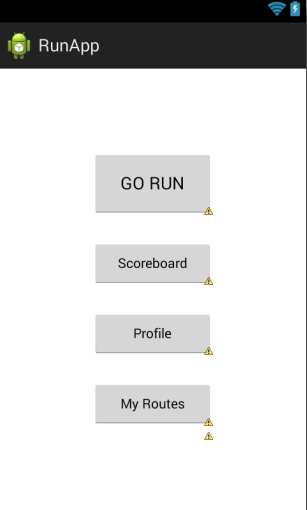
\includegraphics[scale=0.4]{img/mainV1.png}
		\caption{Main Activity Prototype}
		\label{fig:mainV1}
	\end{center}
\end{figure}

There is currently no styling of the buttons, the background or the action bar because this was not part of the focus for this sprint. 

The \texttt{MainActivity} class is implemented with an \texttt{onCreate} function which is part of the activity lifecycle. It runs the initial setup when the activity is first started such as setting the layout of the activity to the \ac{XML}-file producing the layout shown in \autoref{fig:mainV1} and contacting the server. The implementation of the \ac{GUI}, with handling of button clicks, is trivial and will not be explained in further detail, however the \texttt{onCreate} utilizes another class, \texttt{HttpHandler}, to establish a connection to the server, log the user in and get their saved routes. These calls are run on separate threads because network calls are not allowed on the \ac{UI} thread on Android. 

The \texttt{HttpHandler} class has 4 functions: 
\begin{itemize}
	\item{\texttt{is\_reachable} which asserts if the server is reachable and returns a boolean value signifying if it is or not. It instantiates a new socket and attempts to connect via it to the IP and port of the server for 15 seconds, closes the socket and returns the result.}
	\item{\texttt{http\_request} is a generic \ac{HTTP} request function returning a custom \texttt{ResponseData} object consisting of a status code in integers and a response body, which is stored in a string.}
	\item{\texttt{login\_request} is a function taking a username and password as parameters and returning a boolean signifying if the login was successful or not. It adds its received parameters to a list of \texttt{NameValuePair}s and calls \texttt{http\_request} with a \texttt{POST} request and the list as parameters. The \texttt{ResponseData} object is then checked to see that the response has status code 200 and text ``OK'' which means the login was successful.}
	\item{\texttt{route\_request} takes no parameters and returns a \texttt{JSONArray} with the routes the user has saved. It sends a \texttt{GET} request using \texttt{http\_request}. If the response status code is 200 and the status is OK, the array of routes in the \texttt{ResponseData} object resulting from the function call is then saved in a \texttt{JSONArray} object, which is returned.}
\end{itemize}

\subsection{Testing}
The implementation was unit tested to ensure that the functionality worked as intended. For this the jUnit~\citep{junit} test framework and the EMMA~\citep{emma} code coverage tool was used. The focus of the test was on ensuring that correct use of the application resulted in the expected behaviour, thus things like incorrect login credentials was not a part of this test. The tests currently require the server to be running in order to pass.

\subsubsection{Unit tests}
Unit tests were written for 5 of the classes, namely \texttt{Http\-Handler}, \texttt{Main\-Activity}, \texttt{Match\-Comp}, \texttt{Match\-Friend} and \texttt{Run\-Options}. 

For \texttt{HttpHandler} three test were written:

\begin{itemize}
	\item{A check that the server was reachable (this test is a precondition for the others - should it fail, the others will too).}
	\item{A test that a correct \texttt{login\_request} resulted in success }
	\item{A test that a \texttt{route\_request} returned routes.}
\end{itemize}

For the other 4 classes the unit tests were trivial: simulated button clicks on the screen to verify that the correct activities were started. The \texttt{PickRoute} class was not unit tested seeing as testing that activity mere constituted another simulation of an item selection.

\subsubsection{Code Coverage}
The EMMA code coverage tool was employed with the test cases to ensure that they covered a reasonable amount of the code. The results of the coverage tests are shown in \autoref{tab:emma}.

\begin{table}[!ht]
	\centering
	\begin{tabular}{| c | c | c | c |}
		\hline
		\textbf{Class} & \textbf{Method} & \textbf{Block} & \textbf{Line} \\ \hline
		100 \% (13/13) & 80 \% (45/56) & 80 \% (555/689) & 77 \% (148/193) \\
		\hline
	\end{tabular}
	\caption{EMMA Coverage Results}
	\label{tab:emma}
\end{table}

As can be seen the unit tests cover 77 \% of the lines of code and 80 \% of the methods in the tested classes, which we found to be adequate seeing as the untested methods were auto-generated by the \ac{IDE}.
